In this section, we explain the detail of each step in our system. The algorithm 
flow is depicted in Fig.~\ref{fig:system_flow}. First, we load a group of motion 
captured files as the candidate motions. Second, performing the algorithm to 
locate the transition point between motions, then construct the motion graph.
Last, by traversing on the motion graph to generate the infinite and seamless 
motions.

%Fig : system flow
\begin{figure}
\centering
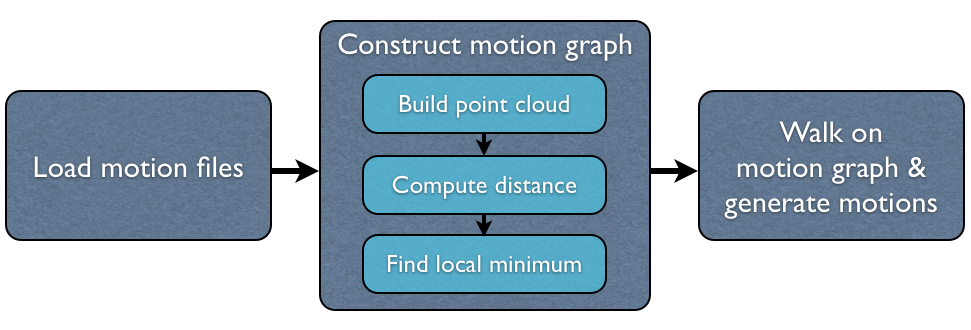
\includegraphics [width=80mm] {Images/flow} 
\caption{Motion graph System flow}
\label{fig:system_flow}
\end{figure}

The remainder of this section is divided into four pars. 
First, we explain the algorithm of detecting candidate transitions between 
motion clips. The following two sections, we discuss about how to blend the 
transition, and synthesize the motion with consistent momentum.
Finally, we explain how to extend the topology to make the virtual character 
looks natural.

\subsection{Detecting Candidate Transitions}
In this section, we discuss about how to locate the transition points between two 
motion clips. 

In~\cite{kovar2002}, they pointed out three issues when measuring the difference between poses at each pair of 
frames: 
\begin{enumerate}
\item Simple vectors norms fail to account for the meaning of the joint angle 
representation.
\item Comparing two motions requires identifying compatible coordinate systems 
instead of rigid 2D coordinate transformation.
\item Smooth blending requires higher-order derivatives of joint transitions.
\end{enumerate}


The similarity metric is defined by calculating the distance $D(A_i,B_j)$ 
between frames $A_i$ and $B_j$. In order to increase vector norms, we measure a 
point as a group of points, called point cloud (see Fig.~\ref{fig:point_cloud}), which is  based on a 
downsampling of the mesh of the character. 
Furthermore, we consider a window of frames length $k$, for $A_i$ to $A_{i+k}$ and $B_{j-k}$ to 
$B_j$. The size of the windows is defined as a third of a second in length, as in~\cite{datadriven}. 

\begin{figure}
\centering
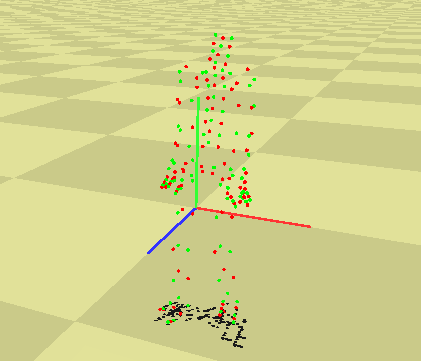
\includegraphics [width=70mm] {Images/point_cloud} 
\caption{Construct the point cloud by down-sampling model}
\label{fig:point_cloud}
\end{figure}

%transform function equation:
\begin {equation}
\min_{\Theta,z_0,z_0} \sum w_i\left \| p_i-T_{\Theta,x_0,z_0}p'_i \right \|^2
\end {equation}

In order to find the closest frames $A_i$ and $B_j$, we may calculate the 
minimum discrepancy of two point cloud $p_i$ and $p'_i$. A rigid transformation $T_{\Theta,x_0,z_0}$
is applied to the second point cloud for transforming the position and rotation 
from second point cloud to the first point cloud. The transformation is important 
to ensure the position and orientation is continuous when blending two poses. 
This transformation has a closed-form solution~\cite{kovar2002}:

%eq1: theta
\begin {equation}
\Theta = arctan\frac{\sum_i (x_i z'_i - x'_i z_i)-\frac{1}{\sum w_i}(\overline{x}\overline{z'}-\overline{x'}\overline{z})}
{\sum_i (x_i z'_i + x'_i z_i)-\frac{1}{\sum w_i}(\overline{x}\overline{z'} +\overline{x'}\overline{z})}
\end {equation}

%eq2: x_0
\begin {equation}
x_0 = \frac{1}{\sum_i w_i} (\overline{x}-\overline{x'}cos\Theta-\overline{z'}sin\Theta)
\end {equation}

%eq3: z_0
\begin {equation}
z_0 = \frac{1}{\sum_i w_i} (\overline{z}+\overline{x'}sin\Theta-\overline{z'}cos\Theta)
\end {equation}

We compute the distance for every pair of frames in our selected motion capture 
database. Therefore, all the pair of frames from motion clip $A$ and $B$ forms a 
2D distance matrix. 
The candidate transition points could be the local minimum error between $A_i$ 
and $B_j$. 
By setting a threshold $\lambda$ to the minimum distance, we can control the quality of the transition 
point to ensure all the transition is capable to blend smoothly.


\subsection{Motion Transition}
After detecting the transition points between two motion clips, we need to 
synthesise the transition motion from $A_i$ to $B_j$. 

The goal of the transition is to interpolate frame $A_i$ to $A_{i+k}$ with frames $B_{j-k+1}$ 
to $B_j$, inclusive. When we calculate the distance $D(A_i,B_j)$, we also keep 
the transformation function. Therefore, the first step is to apply the 
transformation function to motion $B$. 
Then we calculate frame p on the transition ($0\leqslant p < k$), by 
interpolating the root positions and performing spherical linear interpolation 
on joint rotations.

%eq Interpolate R
\begin {equation}
R_p  = \alpha(p)R_{A_{i+p}} + [1-\alpha(p)]R_{j-k+p}
\end {equation}

%eq slerp
\begin {equation}
q^i_p = slerp(q^i_{A_{i+p}}, q^i_{B_{j-k+p}}, \alpha(p))
\end {equation}

Whre the $R_p$ is the root position at interpolated frame $p$ and $q^i_p$ is the 
$bone^i$'s rotation at interpolated frame $p$. To attain the consistent 
continuity of the motion, we use the blending weight $\alpha(p)$ to interpolate 
frame $A_{i+p}$ to $B_{j-k+p}$:

%how to calculate p
\begin {equation}
\alpha(p) = 2(\tfrac{p+1}{k})^3-3(\tfrac{p+1}{k})^2+1, -1<p<k
\end {equation}

When a user wants to change the character's action, we can walk on the graph by a shortest path. 
In order to decrease time complexity, instead of using all-pairs shortest algorithm 
(Floyd-Warshall), we use Bellman-ford algorithm with time complexity $O(\left \| V \right \| \left \| E \right \|)$.
%bellman-ford : label*||V||*||E||

After precompute all shortest path from node to node, we keep the outbound edges 
and the path to a certain label of the node (see Listing.1).
The motion frame and label is from the origin motion clip. The outbound edges 
keeps all the outbound edge of the node for traversing the graph. The label paths 
only keep the next edge of the route to a certain label. 

\begin{lstlisting}[label=transition_node_code,caption=Data structure of Transition Node]
struct {
  int id;
  int motion_frame;
  int label;
  Vector outbound_edges;
  Vector label_paths;
} Transition_Node;
\end{lstlisting}
%\caption {The data structure of a transition point}

For Edge (see Listing.2), we keep the both ends of the Transition node, animated motion, translation $[x_0, z_0]$ and the rotation 
$\Theta$. Every time when transiting to a edge, we need to apply the 
transformation to the root position of the motion to ensure the position and 
orientation is continuous. 

\begin{lstlisting}[label=edge_code,caption=Data structure of Edge]
struct {
  int id;
  int src_node;
  int dest_node;
  double theta, x_0, z_0;
  Motion* motion;
} Edge;
\end{lstlisting}
%\caption {The data structure of an edge on motion graph}

%\subsection{Consistent Momentum between Motions}
%Due to we can't get the motion capture files they are consistent in the 
%momentum, it's required to synthesise the motion with the same momentum or even 
%exaggerate the motion to make it looks powerful in the fighting.

\subsection{Infinite Motion Graph}
In order to make the character looks alive, we introduce the rest motion to make 
the character can transit to rest motion if the user doesn't give any command.
Now each segment is manually given a label for identifying the action types.
When we are walking on the graph, we can set the target label, and try to find 
a shortest path to reach the target label. After arriving the target label, 
keep selecting the closest segment withe the same label. 
Fig.~\ref{fig:graph} shows the constructed motion graph with connecting to rest motion. 
When reach the end of the segment of a label, in order to prevent the character 
stop acting, we set the next target label as rest pose to keep it acting all the 
time. The rest pose is connected to the both ends of each motion, to maintain 
a cycle for every motions. In our implementation, we cycle the walking and running into a infinite loop to 
keep the character walking/running. 

% a graph picture

\begin{figure}
\centering
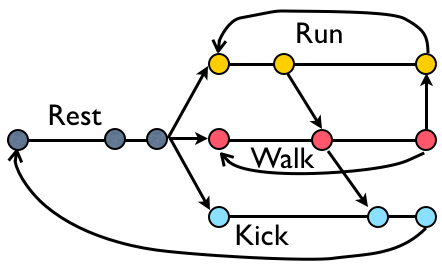
\includegraphics [width=70mm] {Images/graph} 
\caption{Traversing on the motion graph. Each color represents a label; grey is rest motion, yellow is running, red is walking, and blue is kicking. }
\label{fig:graph}
\end{figure}
